%!TEX root = ../main.tex
% What is the project about? 
% What problem are you tackling? 
% What is your research question? 
% Why do these problems need solutions? Why are they important?
% What is the background to the problem? Who is the client? What do they want?
% What existing methods have been tried? How has I.T. been applied so far? 
% What constraints do you have? (Time, PCs, money, users, software etc) 
% What is the scope of what you have set yourself to do. What is not included?
% What broad approach was taken? (Summarise your broad approach the project) 

\chapter{Introduction}
\label{chap:intro}
We live in a world where mobile development dominates, a world in which mobile phones are always with us to enhance our everyday lives, to give information, simplify tasks and provide entertainment. With the increase of mobile application called apps, individuals are seeking information on the go, this need allows developers to tailor make apps targeting exact needs of the users. Correlating this, Google play store and the iOS Store has more than 5 million apps (data from statista).

According to Statista 197 billion of mobile apps were downloaded in 2017, furthermore, 2.53 billion people use a smart phone, a report from Ofcom, confirms 55\% of mobile owners uses their mobile phone to visit social networking sites or apps. 
Keeping this statistic in mind and with the increase of use of mobile application, it is not surprising to see an increase in the creation of app designed purposely for events.

Event apps offer information attendees needs, such as schedule, maps, date, time and more. Attendees download these apps so they can access information about any event they are interested in.

If we go back about 10 years ago, think how events where published, what comes to mind is a flyer. That old flyer, not designed properly, with no or less information printed on it and with all that typo(as once printed the organizer has no way of amending it). Yes exactly, those tedious flyers, that once received you will probably not even read and just bin.  

Furthermore, if you are interested in that event, you will be handed that large paper with all critical information in it, address, date, event information and more, hoping it will not get lost in a mass of other papers.

Point is, mobile app illustrate the advancement society has made when it comes to tech, and for now this research is based on the development of user friendly Android based application named Univent. This event app will aid users in finding any upcoming events on campus and help event organizers to have a unique platform to publish their events and activities.
This thesis will describe the design, development and evaluation of an app that will be used as a platform to publish any upcoming event in the University, helping people to interactively engage in activities and events going on in campus.

\section{Background \& Context}
Based on observation, students find it quite difficult to advertise upcoming events in University, with the only way being distribution of flyers around and most of these ending up in bins. It is quite difficult as well if the target is to reach as many students as possible within a short space of time. Flyers normally lack long term impact as many students may read the leaflet and then discard them. Most students that receive flyers will look at it once and if not interested will bin the leaflet as it's not worth keeping. Therefore, they might not have anything to remind them of the event or service being advertised.
 
Furthermore, we live in a generation which likes to get information about activities on campus very easily, without carrying around flyers of any sort. 

Moreover, the use of flyers affects the target, in that, to reach as many people as possible, for instance there might be University students who are interested in a particular event, but since they were not there at that moment of distributing the flyer they will not have the opportunity to know about the event. This will mean the individual will be unable to participate and they will not gain the benefit that event offered, this miss out on the opportunity of meeting new people for example.

\section{Problem Definition}
\label{prob_def}
Whilst the 21st century digital world offers modern techniques, that can reduce cost, unfortunately flyers and leaflet distribution is still popular in Bournemouth University(BU). This form of advertisement, also known as leafleting, though may have quite an advantage because it’s easy to read, as the design of a leaflet tend to have larger letters and a limited number of words, as a fact they are designed predominantly to attract attention, not to go into too much detail.

\textbf{Limited Target:} the number of people reached is limited as this depends on the number of flyers that can physically be delivered. 

Flyers have a trend to become obsolete, as people often order large quantities because  higher quantity equals lower cost and there is a tendency of printing more material than needed for this reason. As events or services being promoted on the leaflets don’t last forever, it is quite important to distribute all brochure before the end date because discarding the remaining leaflet is a waste of money and paper.

Another main issue is the mistakes that can easily be made in print work, and when flyers are already printed out, this will turn into an extra cost to amend.

In our current era of tech, flyers is not the best way of publishing an event. It includes a long process to create a simple leaflet, finding words which are more compelling to your message, have a design, print and distribute the flyers. This process takes a long time and a lot of money if the leaflet needs to look professional, which consequently means working with a design company, photographer or a graphic artist. This often ends up being an arduous and expensive process.

Another disadvantage is that they are most often dismissed by people as \say{mere sheet of paper} according to an article at brochuremonsters.com. Complacency viewed by individuals as annoying, for those who don’t want to chat and don’t have time to stop and listen, to what is being advertised as they will rather do it in their own time. One might also glance at it for a second, but if it doesn’t spark any immediate interest it will end up in the nearest bin.

\say{This is very alarming as often it will end up as waste, and the main reason is that people are receiving leaflet they don’t want to receive}, said Ryan O’Quin, membership \& development with the Ecology Action Centre in Halifax. Reducing the use of this form of advertisement will help the environment through the reduction of paper waste. 

\section{Solution}
\subsection{Existing solution}
 Though there is a vast market for event applications with the purpose of organising social functions and activities, there is always scope for more innovative ideas.

This thesis will seek to examine several existing event applications in section \ref{similar_app}.

\subsection{Proposed solution}
This project aims to create a paperless solution where information is always available and easy to access. With this solution students will rely on mobile application, allowing them to read or post any ongoing or upcoming events (club nights, parties, football matches, university events, external speakers, etc.).

Let's consider the amount of time it takes to prepare flyers, create a design, decide on content, print and distribute, all of this is time consuming, and if you want the leaflet to look professional, this means hiring a marketing or design firm.

Flyers can be labour intensive and costly to produce and distribute especially if targeting a large audience and it’s very difficult sometimes to build a connection with a target who are always on the go. The number of people reached by flyers are very limited as this is highly dependant on the number of flyers you can distribute to the audience. It is also quite an arduous process, from design, printing and finding the perfect location to reach as many people as possible. 

Another disadvantage is the finality of print compared to an app, once a poster is printed it is more difficult to make corrections or adaptions and it is therefore less flexible in its adaptability when compared to a software presentation that can be modified any time.  

This is where a paperless solution for flyers has a powerful advantage. This minimizes your expenses, as there is no need to pay for printing and there is no need to worry about losing information, which can be accessed everywhere.

The application aims to provide the latest event on users mobile phone with all features designed to work online to give the latest information to users, and improve the event experience in every aspect: it is designed to build stronger connection for attendee satisfaction, a comprehensive event search to look for any interested event, have a customized event dashboard displaying only events of interest and more.

This application not only provides easy to access information to attendees, it helps organizers plan events, create the event, publish it and keep track of the number of attendees.

By providing all the benefit, and useful features of the application, it should show how essential it is to have a unique mobile platform for universities where events can be posted, minimizing effort and maximizing benefit to all attendees and event planners.

\section{The Challenge}
\label{the_challenge}
With the number of prospective students who use smartphone steadily increasing, along with internet usage, Universities are improving student experience and enabling them to see exactly what’s happening at the university and feel part of a wider community through use of tech. BU has already embraced social media and new technologies to engage its students through channels like, Facebook, Twitter, BU app, etc.

The embracement of tech is further illustrated with BU own app, which enables students to find numerous information from checking their timetable to downloading lectures and seminars.

Infact it will be brilliant for this app the author has developed to be taken on board by the university and incorporated in the BU mobile app, as often integrating other apps on an internal system will be a challenge but as Doug Poole, digital media officer at Southampton University stated, -\say{it is worth persevering and joining these systems up as that is when the user will experience genuinely useful functionality}.

\section{Target Audience}
The main users of this mobile application will be everyone on the faculty. This is mainly designed to aid students and everyone at university to be aware of any ongoing activities or events at the university and help event organizers to have an easy platform to publish any activity they have organized. The app has a register and login feature which only accepts university emails, validates the user login details and checks a university email domain. This is one of the main feature of the app as it focuses solely on the University events and any other activities posted by students, this makes the app unique as all the similar mobile applications are targeted at a broader range of audience.

\section{Project Aims}
The application aims are to solve the problem mentioned above. To achieve this, the project must inspire and convince users away from printing out flyers or brochures and make it easier for students to post any upcoming events and reach as many audience as possible through the use of the app. Lecturers can post important events (external speaker etc.) and the University can post any important upcoming events. This project will make it much easier for people to connect and make each other aware of any events ongoing or upcoming events, through easy accessibility on their mobile phones. All these features are designed to work online to give the latest information to users and improve the event experience in every aspect.

\section{Project Objective}
The thesis objective should formulate a means to providing a solution to the problem, this following objective have been set out to fulfil this aim:
\begin{itemize}
\item To elicit requirements from observation
\item Provide a solution that helps users to keep track of activities in the faculty and aid them in publishing any new ones. 
\item Design front end system that will show JSON data retrieved from server.
\item App must work without delays and have smooth transaction 
\item Final project must work without issues, ensuring user safety  	
\end{itemize}

\section{Risk}
Risk in software project incorporates various factors or conditions that may represent an issue for the completion of the project. Risk can be divided into two component; the likelihood the risk will occur and the impact of the risk. 

Managing risk includes identifying any potential risk, verify the impact on the functionality and come up with a strategy to control it.
\begin{figure}[h]
	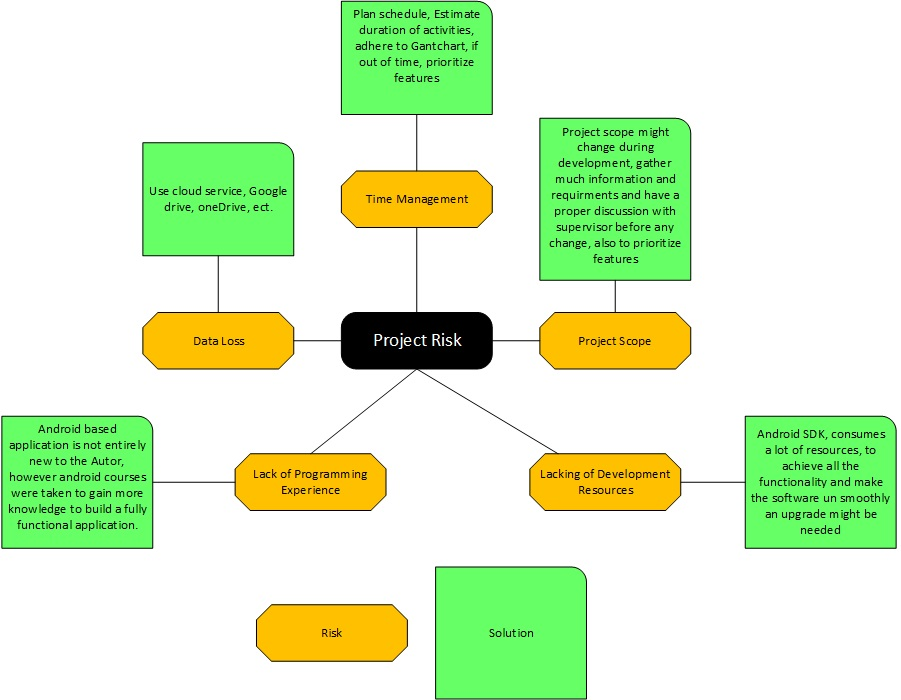
\includegraphics[width=0.6\textheight]{risk}	
	\caption{Risk Diagram}
	\label{fib:risk}
\end{figure}

\newcolumntype{L}[1]{>{\raggedright\let\newline\\\arraybackslash\hspace{0pt}}m{#1}}
\newcolumntype{C}[1]{>{\centering\let\newline\\\arraybackslash\hspace{0pt}}m{#1}}
\newcolumntype{R}[1]{>{\raggedleft\let\newline\\\arraybackslash\hspace{0pt}}m{#1}}

\begin{longtable}{| L{3cm} | L{3cm} |}
  Likelihood  & Impact  \\ \hline
	P = Possible &	M = Major\\	\hline
	U = Unlikely &	Me = Medium\\	\hline
	L = Likely   &	Mi = Minor\\	\hline
	V = Very Likely  &	N = No Impact\\	\hline
	\caption{Likelihood and Impact}
	\label{Likelihood_Impact}
\end{longtable}
\pagebreak
	
\begin{longtable}{| c | L{3cm} | L{3cm} | L{3cm} | L{3cm} |}
	Risk ID  & Risk & Impact & Likelihood & Solution \\			\hline
	1 & Project Scope &  Me   &  L  & Project scope might change during development, gather much information and requirments and have a proper discussion with supervisor before any change, also to prioritize features \\
	
		\hline
			2 & Time Management & Mi  & V  & Plan schedule, Estimate duration of activities, adhere to Gantchart, if out of time, prioritize features \\
		
			\hline
		3 & Lacking of Development Resources & M & P  & Android SDK, consumes  a lot of resources, to achieve all the functionality and make the software un smoothly an upgrade might be needed\\
		
			\hline
		4 & Lack of Programming Experience & Me	& L & Android based application is not entirely new to the author, however android courses were taken to gain more knowledge to build a fully functional application.  \\
		
			\hline
		5 & Data Loss &	M & V  & Use cloud service, Google drive, oneDrive, ect. \\	
			\caption{Risk Analysis}
		\label{risk_analysis}
\end{longtable}

\section{Achievement}
A mobile android application has been developed successfully and ready to go on the market.  All requirements are met, and it has been tested by both client and developer and all necessary tests have been executed. The project accomplishes the following objectives:
\begin{itemize}
	\item All functionality is integrated and working efficiently
	\item Multiple actions can be performed on the app
	\item App is pusblished and can be downloaded from the Google Play Store Market
\end{itemize}

\section{Android vs iOS}
This section explains the main operating systems on the market, those being Android and iOS, see Appendix \ref{androidvsios}

\section{Success Criteria}
\label{success_criteria}
The measure of success can be judged on whether the project as a whole offers a solution to the aforementioned problem. The app's functionality will be assessed throughout the entire software development lifecycle, in the form of debugging and running the application on a mobile device. Meeting with potential clients will provide feedback that will aid in verifying most of the functionalities which may well lead to changes in the features and appearance of each component. The main feature of the app is to provide support in publishing and keeping track of activities in the faculty, therefore the app will be uploaded on the play store, to enable users to download and leave comments regarding their experience of using the app which will allow collation of what feedback that can be utilised to gauge the overall success of the app and allow the developer to improve any areas of concerns relating to the main function of the app.

